\chapter{Progettazione e codifica}
\label{cap:progettazione-codifica}

\intro{Il capitolo inizialmente presenta gli strumenti e le tecnologie analizzate e utilizzate per la realizzazione del prodotto. Successivamente si vede l'effettiva creazione delle classi del progetto, affiancate da una struttura preesistente fondamentale per le classi che offre affinché il modulo funzioni e svolga la sua funzione. }\\

\section{Tecnologie e strumenti}
\label{sec:tecnologie-strumenti}

Di seguito viene data una panoramica delle tecnologie e strumenti utilizzati.

\subsection*{HTML5}
Tecnologia standard per la creazione di pagine web. È studiata e conosciuta con il corso di Tecnologie Web.

\subsection*{CSS}
Tecnologia standard per la creazione di pagine web e il loro abbellimento. Fornisce una vasta gamma di funzionalità per la personalizzazione delle pagine. È studiata e conosciuta con il corso di Tecnologie Web.
\subsection*{Bootstrap3/5}
Bootstrap è un framework che fornisce delle classi le quali raggruppano uno o più attributi del css, per la creazione di pagine web \textit{responsive\gls}. \\
Bootstrap è utilizzato nello stile \textit{inline} di \textit{HTML} e le sue classi vengono inserite all'interno del \textit{tag\gls} "class" di HTML di un elemento. In questo modo, specificando la classe di Boostrap che si vuole utilizzare, verrà applicato un certo stile all'elemento selezionato. Si possono concatenare più classi per un certo elemento.\\
La differenza tra le due versioni di \textit{Boostrap} 3 e 5 è nella gamma di funzionalità che offrono. La versione 5 è la più recente e molte più funzionalità di quelle precedenti, adattandosi alle nuove feature di \textit{HTML5}. \\
Ad oggi si cerca di migrare dalle versioni più vecchie a quella più recente.
\subsection*{Servlet}
Le \textit{servlet} permettono di soddisfare delle \textit{request\gls} \textit{HTTP\gls} proveniente da web. Ogni servlet viene richiamata e caricata una sola volta e poi resta in memoria per rispondere alle chiamate successive. 
\subsection*{JSP}
Le \textit{JavaServer Page} rappresentano una tecnologia fondamentale per la realizzazione di pagine web dinamiche. Infatti forniscono dei \textit{tag} speciali con i quali possono essere richiamate delle funzioni specifiche in modo da rendere la pagina dinamica. I file \textit{JSP} sono caratterizzati dell'estensione .jsp e costituiscono le vere e proprie pagine web visualizzate dall'utente in quanto permettono la codifica in \textit{HTML} e \textit{XML}.
\subsection*{JSTL}
\textit{JavaServer Pages Standard Tag Library} è una libreria che estende JSP offrendo nuove funzionalità per applicazioni web in \texit{JAVA EE}. 
\subsection*{Apache Struts}
\textit{Apache Struts} è un \textit{framework oper-source} che supporta lo sviluppo di applicazioni web in Java con il pattern MVC. Infatti \textit{Struts} ha il compito di organizzare le richieste del client e richiamare le funzionalità della logica di business. \\
Il framework è composto da tre elementi principali:
\begin{itemize}
\item \textit{Request Handler\gls}: viene mappato ad un URI dallo sviluppatore;
\item \textit{Response Handler\gls}: la risposta verrà passata ad un'altra risorsa che la completerà;
\item \textit{Tag}: aiutano lo sviluppatore per lo sviluppo.
\end{itemize}

\noindent
Per configurare tutti i collegamenti tra i vari elementi e le loro interazioni si utilizza il file \textit{\textbf{struts.xml}}. In questo file vengono specificati anche gli \textit{\textbf{interceptor}} per le \textit{Action} delle nostre classi. La specifica degli \textit{interceptor} è una fase importante dello sviluppo di un'applicazione web.

\subsection*{JQUERY Taconite}
\textit{JQUERY Taconite} permette di aggiornare \texit{DOM} multipli utilizzando il risultato di una singola chiamata \textit{AJAX\gls}. \\
Viene generato un \textit{XML} con le istruzioni per l'aggiornamento dei diversi \textit{DOM}

\subsection*{Hibernate}
È un framework che permette di mappare gli oggetti del modello ad un \textit{database} relazionale. Lo sviluppatore non deve preoccuparsi di implementazione ma è \textit{Hibernate} che si occupa del collegamento al database e di eseguire le operazioni \textit{CRUD\gls}, andando a generare query e leggerne il risultato.

\subsection*{Spring}
\textit{Spring}\gls è un framework volto ad aiutare lo sviluppo di applicazioni più o meno complesse attraverso la sua architettura modulare. Spring è diviso in cinque livelli e in questo modo si possono escludere le parti non necessarie per l'applicazione.\\
L'elemento principale di \textit{Spring} è il \textit{Core Container} che ha il compito di creazione e gestione di tutti gli oggetti dell'applicazione, detti anche \textit{\textbf{beans}\gls}.
\subsection*{Wro4j}
\textit{Wro4j} è uno strumento per l'ottimizzare le risorse web e velocizzare il caricamento delle pagine. Il suo compito è quello di organizzare le risorse, come i file \textit{css} e \textit{js}, raggrupparli e farli scaricare tutti in una sola volta alla pagina web.\\
Normalmente un browser può scaricare al massimo due risorse contemporaneamente e questo limite porta ad un caricamento della pagina lento in vista di molte risorse da scaricare. \textit{Wro4j} elimina questo problema comprendendo tutte le risorse in un'unica risorsa.
\subsection*{SVNKit}
\textit{SVNKit} è uno \textit{toolkit} \textit{Open-Source} e permette l'accesso il remoto e in locale a delle \textit{repository} per le applicazioni Java. Funge anche da sistema di versionamento. 

\subsection*{Apache Maven}
\textit{Apache Maven} è uno strumento per la gestione delle dipendenze tra un progetto Java e le versioni delle librerie che servono e si occupa anche di effettuare il download di tali risorse. \\
Le relazioni tra progetto e librerie sono definite in un file \textit{XML} chiamato \textit{\textbf{POM}}.

\subsection*{Apache Tomcat}
\textit{Apache Tomcat} è un server web che permette l'esecuzione di applicazioni web. Supporta le specifiche di \textit{JSP} e \textit{servlet}.\\
Esistono diverse versioni per i server \textit{Tomcat} e si può scegliere la versione che offre le funzionalità giuste per la propria applicazione.
\subsection*{DBeaver}
È un'applicazione che si occupa di gestire i database. Si possono creare nuovi database, creare tabelle, manipolare i dati, ecc...

\section{Progettazione}
\label{sec:progettazione}
La fase di progettazione è una fase cruciale per la realizzazione del progetto. Prima ancora di iniziare la progettazione del lavoro assegnato è importante analizzare l'ambiente già esistente, capirne il funzionamento e individuare se ci sono elementi che potrebbero servire al nostro scopo. \\
Una tecnica per una buona progettazione è concentrarsi su un elemento alla volta. Prendere in considerazione tutti gli elementi del progetto potrebbe sembrare più efficace e veloce, ma così facendo si può perdere il focus della funzione delle classi del prodotto.\\ 
Quindi l'idea è quella di analizzare e progettare una singola classe, vedere se funziona correttamente e da lì procedere ed andare avanti con lo studio per la realizzazione della prossima classe.




\subsection{Base di Dati}
Per la progettazione della base di dati si è partiti da una struttura già esistente nell'azienda e si sono inseriti i nuovi elementi del progetto. Si è eseguito un \textit{refactoring} di alcune delle tabelle preesistenti per correggerle ed adattarle a quelle nuove, senza però modificarne attributi fondamentali per le altre parti della webapp. Anche qui c'è stato allora una fase di profonda e attenta analisi per avere una base di dati consistente. 
\subsubsection*{Tabelle preesistenti}
Il progetto utilizza tabelle preesistenti per il suo scopo. Le tabelle sono: 
\begin{itemize}


    \item \textbf{Cliente}: questa tabella rappresenta l'entità cliente e ha tutti gli attributi necessari per definirne lo scopo all'interno della webapp. Il cliente non è la singola persona ma bensì l'azienda a cui poi saranno collegati sia i dipendenti sia i progetti richiesti da questa. Gli altri attributi presenti servono per le altre parti della webapp
    \item \textbf{User}: gli user sono tutte le persone coinvolte nell'azienda, interne ed esterne. Quindi troveremo sia il personale di CWBI sia il personale delle aziende clienti.
    \item \textbf{Progetto}: questa tabella rappresenta un progetto dell'azienda. Avrà tutti gli attributi necessari e sarà collegata ad un cliente. Un progetto può essere collegato a più aziende diverse.
    \item \textbf{ProgettoCliente}: questa tabella rappresenta la relazione tra progetto e cliente. Viene chiamata in causa quando si dovrà scegliere l'azienda e il progetto su cui si vorrà aprire il ticket.
        \item \textbf{ProgettoUser}: questa tabella rappresenta la relazione tra progetto e user. Ogni progetto può avere associato uno o più utenti.
\end{itemize}

\subsubsection*{Tabelle introdotte}
\begin{itemize}
	\item \textbf{Ticket}: questa tabella rappresenta l'entità ticket con tutti gli attributi che lo caratterizzano. Sarà collegata all'entità ProgettoCliente in quanto il ticket sarà aperto per uno specifico progetto di una specifica azienda.
	
	\item \textbf{TicketItem}: questa tabella rappresenta i commenti presenti in ogni ticket. Un commento potrà avere un solo ticket di riferimento, cioè quello in cui è stato scritto.
\end{itemize}


\begin{figure}[H]
\bigskip
\bigskip
\bigskip
\bigskip
    \centering 
    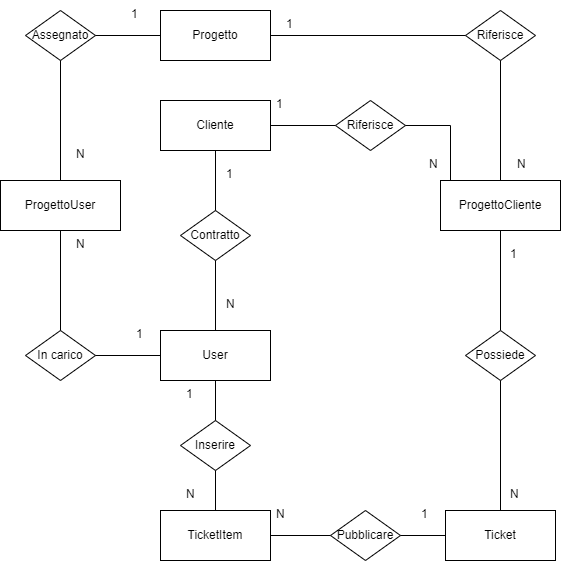
\includegraphics[width=1.1\columnwidth]{diagrammaBase} 
    \bigskip
    \caption{Base di Dati - Relazioni delle tabelle del progetto}
\end{figure}

\newpage

\begin{figure}[H]
\bigskip
\bigskip
\bigskip
\bigskip
\bigskip
    \centering 
    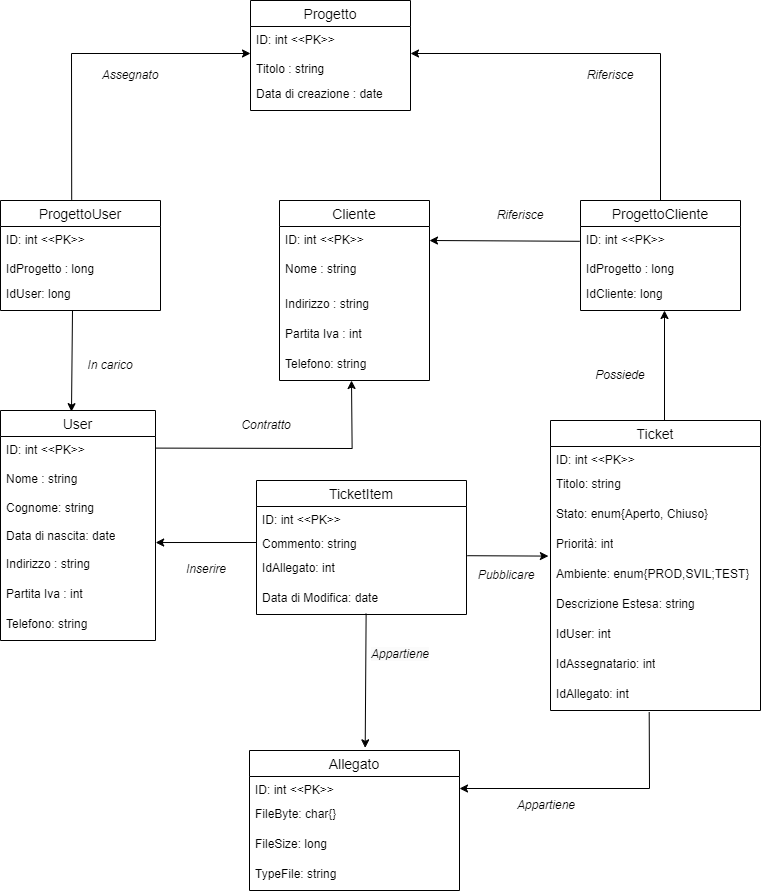
\includegraphics[width=1.1\columnwidth]{diagrammaEvoBase} 
    \bigskip
    \caption{Base di Dati - Tabelle del progetto}
\end{figure}
\newpage

\subsubsection*{Analisi delle tabelle}
            \begin{table}[H]
                \centering
                \renewcommand{\arraystretch}{1.8}
                \renewcommand\tabularxcolumn[1]{m{#1}}
                \begin{tabularx}{0.9\textwidth} {
                    >{\hsize=.8\hsize\linewidth=\hsize}X
                    >{\hsize=1.2\hsize\linewidth=\hsize}X}
                    \textbf{Cliente}\\
                    \hline
                    \textit{Id} & Identificativo univoco di ogni cliente. \\
                    \hline
                    \textit{Nome} & Nome dell'azienda.  \\
                    \hline
                    \textit{Indirizzo} & Indirizzo della sede principale dell'azienda. \\
                    \hline
                    \textit{Partita Iva} & Partita Iva dell'azienda \\
                    \hline
   	                \textit{Telefono} & Telefono dell'azienda \\
                    \hline
                \end{tabularx}
                \smallskip
                \caption{Tabella Cliente}
            \end{table}
            \smallskip
 \begin{table}[H]
                \centering
                \renewcommand{\arraystretch}{1.8}
                \renewcommand\tabularxcolumn[1]{m{#1}}
                \begin{tabularx}{0.9\textwidth} {
                    >{\hsize=.8\hsize\linewidth=\hsize}X
                    >{\hsize=1.2\hsize\linewidth=\hsize}X}
                    \textbf{ProgettoCliente}\\
                    \hline
                    \textit{Id} & Identificativo univoco di ogni ProgettoCliente. \\
                    \hline
                    \textit{IdProgetto} & Id del progetto a cui si riferisce.  \\
                    \hline
                    \textit{IdCliente} & Id dell'azienda a cui si riferisce. \\
                    \hline
                \end{tabularx}
                \smallskip
                \caption{Tabella ProgettoCliente}
            \end{table}
            \smallskip
 \begin{table}[H]
                \centering
                \renewcommand{\arraystretch}{1.8}
                \renewcommand\tabularxcolumn[1]{m{#1}}
                \begin{tabularx}{0.9\textwidth} {
                    >{\hsize=.8\hsize\linewidth=\hsize}X
                    >{\hsize=1.2\hsize\linewidth=\hsize}X}
                    \textbf{Progetto}\\
                    \hline
                    \textit{Id} & Identificativo univoco di ogni Progetto. \\
                    \hline
                    \textit{Titolo} & Titolo del progetto.  \\
                    \hline
                    \textit{Data di creazione} & Data in cui è stato aperto il progetto. \\
                    \hline
                \end{tabularx}
                \smallskip
                \caption{Tabella Progetto}
            \end{table}
            \smallskip

 \begin{table}[H]
                \centering
                \renewcommand{\arraystretch}{1.8}
                \renewcommand\tabularxcolumn[1]{m{#1}}
                \begin{tabularx}{0.9\textwidth} {
                    >{\hsize=.8\hsize\linewidth=\hsize}X
                    >{\hsize=1.2\hsize\linewidth=\hsize}X}
                    \textbf{ProgettoUser}\\
                    \hline
                    \textit{Id} & Identificativo univoco di ogni ProgettoUser. \\
                    \hline
                    \textit{IdProgetto} & Id del progetto a cui si riferisce.  \\
                    \hline
                    \textit{IdUser} & Id dell'utente a cui si riferisce. \\
                    \hline
                \end{tabularx}
                \smallskip
                \caption{Tabella ProgettoUser}
            \end{table}   
                 
    			\smallskip 
            \begin{table}[H]
                \centering
                \renewcommand{\arraystretch}{1.8}
                \renewcommand\tabularxcolumn[1]{m{#1}}
                \begin{tabularx}{0.9\textwidth} {
                    >{\hsize=.8\hsize\linewidth=\hsize}X
                    >{\hsize=1.2\hsize\linewidth=\hsize}X}
                    \textbf{User}\\
                    \hline
                    \textit{Id} & Identificativo univoco di ogni User. \\
                    \hline
                    \textit{Nome} & Nome dell'utente.  \\
                    \hline
                    \textit{Cognome} & Cognome dell'utente.  \\
                    \hline
                     \textit{Data di nascita} & Data di nascita dell'utente.  \\
                    \hline
                    \textit{indirizzo} & Indirizzo dell'utente.  \\
                    \hline
                    \textit{Partita Iva} & Partita Iva dell'utente \\
                    \hline
   	                \textit{Telefono} & Telefono dell'utente \\
                    \hline
                \end{tabularx}
                \smallskip
                \caption{Tabella User}
            \end{table}
            \smallskip 
            
 \begin{table}[H]
                \centering
                \renewcommand{\arraystretch}{1.8}
                \renewcommand\tabularxcolumn[1]{m{#1}}
                \begin{tabularx}{0.9\textwidth} {
                    >{\hsize=.8\hsize\linewidth=\hsize}X
                    >{\hsize=1.2\hsize\linewidth=\hsize}X}
                    \textbf{Ticket}\\
                    \hline
                    \textit{Id} & Identificativo univoco di ogni Ticket. \\
                    \hline
                    \textit{Titolo} & Titolo del ticket.  \\
                    \hline
                    \textit{Stato} & Stato del Ticket. \\
                    \hline
                    \textit{Priorità} & Priorità che un ticket ha. Parte da un minimo di 1, quindi poco urgente, ad un massimo di 4, urgente. \\
                    \hline            
            
                 \end{tabularx}
                \smallskip
                \caption{Tabella Ticket}
            \end{table}  
            
 \begin{table}[H]
                \centering
                \renewcommand{\arraystretch}{1.8}
                \renewcommand\tabularxcolumn[1]{m{#1}}
                \begin{tabularx}{0.9\textwidth} {
                    >{\hsize=.8\hsize\linewidth=\hsize}X
                    >{\hsize=1.2\hsize\linewidth=\hsize}X}
                    \hline
                    \textit{Ambiente} & Ambiente del Ticket. Un ticket può essere aperto in base all'ambiente in cui si sta testando l'applicazione e si trova il problema. Si hanno tre diversi ambienti: PROD, SVIL, TEST.\\
                    \hline
                    \textit{Descrizione} & Descrizione del Ticket. Utile per approfondire il problema che si è riscontrato.\\
                    \hline
                    \textit{IdUser} & Id dell'utente che ha aperto il ticket. \\
                    \hline
                    \textit{IdAssegnatario} &  Id dell'utente a cui è stato assegnato il ticket. Può essere cambiato durante il ciclo di vita del ticket. \\
                
                    \hline
                   \textit{IdAllegato} &  Id dell'allegato caricato al ticket. Può essere cambiato durante il ciclo di vita del ticket. \\
                
                    \hline
                \end{tabularx}
                \smallskip
                \caption{Tabella Ticket}
            \end{table}   
                 
    			\smallskip      

 \begin{table}[H]
                \centering
                \renewcommand{\arraystretch}{1.8}
                \renewcommand\tabularxcolumn[1]{m{#1}}
                \begin{tabularx}{0.9\textwidth} {
                    >{\hsize=.8\hsize\linewidth=\hsize}X
                    >{\hsize=1.2\hsize\linewidth=\hsize}X}
                    \textbf{TicketItem}\\
                    \hline
                     \textit{Id} & Identificativo univoco di ogni Commento. \\
                    \hline
                    \textit{Commento} & Contenuto del commento. \\
                    \hline
                    \textit{IdAllegato} & Id dell'allegato caricato al commento. \\
                    \hline
                    \textit{Data di Modifica} & Data in cui è stato modificato il ticket. \\
                    \hline
                \end{tabularx}
                \smallskip
                \caption{Tabella TicketItem}
            \end{table}
            \smallskip
            
 \begin{table}[H]
                \centering
                \renewcommand{\arraystretch}{1.8}
                \renewcommand\tabularxcolumn[1]{m{#1}}
                \begin{tabularx}{0.9\textwidth} {
                    >{\hsize=.8\hsize\linewidth=\hsize}X
                    >{\hsize=1.2\hsize\linewidth=\hsize}X}
                    \textbf{Allegato}\\
                    \hline
                    \textit{FileByte} & Contenuto del file caricato codificato in un vettore di caratteri (char[]) \\
                    \hline
                    \textit{FileSize} & Dimensione del file caricato. \\
                    \hline
                    \textit{TypeFile} & Tipo del file caricato. \\
                    \hline
                \end{tabularx}
                \smallskip
                \caption{Tabella Allegato}
            \end{table}
            
\newpage
\subsection{Architettura}
Lo sviluppo dell'applicazione avviene secondo il \textit{pattern} architetturale \textbf{MVC \glsfirstoccur} (\textit{Model - View - Controller}). \\
Questo \textit{pattern} permette di dividere e rendere modulabile l'applicazione.
\begin{itemize}
\item \textbf{Model}: si occupa della gestione dei dati, del salvataggio delle risorse e della logica di business;
\item \textbf{View}: si occupa di visualizzare i dati salvati nel modello, presentandoli secondo una schema definito.
\item \textbf{Controller}: ha il compito di gestire la comunicazione tra il modello e la vista ed elaborare gli input dell'utente per poi fornire in output un determinato risultato.
\end{itemize}

\begin{figure}[H]
    \centering 
    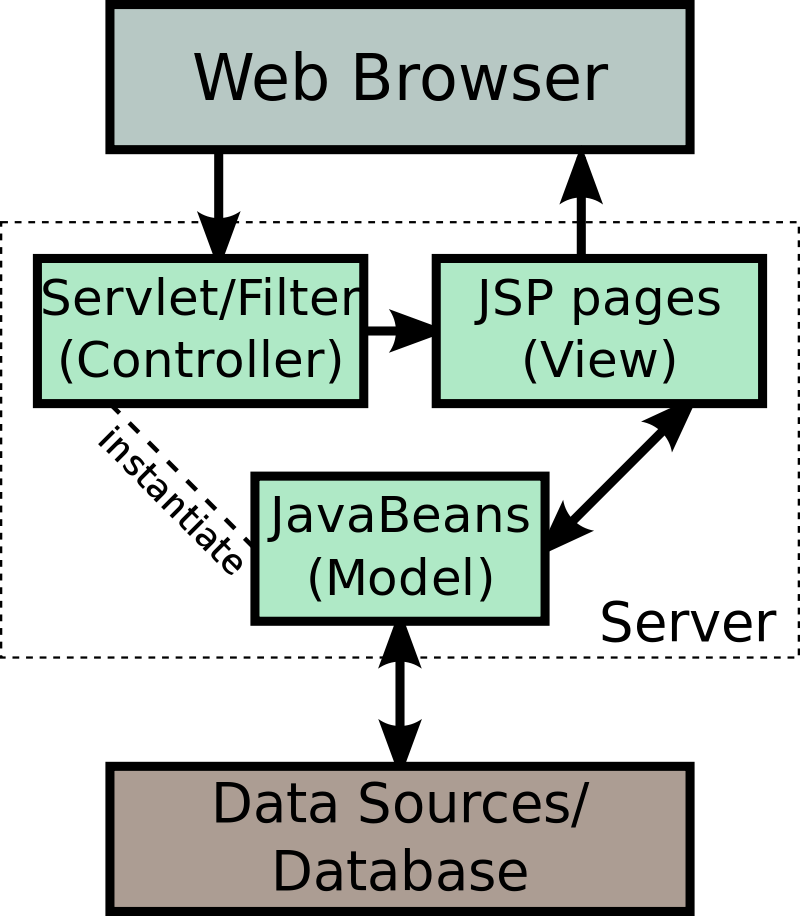
\includegraphics[width=0.4\columnwidth]{MVC} 
    \bigskip
    \caption{Schema MVC}
\end{figure}

\noindent
Utilizzare il pattern \textit{MVC} permette di avere dei \textbf{vantaggi}:
\begin{itemize}
\item \textbf{Manutenzione}: la suddivisione in componenti rende la manutenzione dell'applicazione più semplice, andando a concentrarsi sulla parte interessata.  
\item \textbf{Scalabilità}: con l'aumentare delle esigenze l'applicazione richiederà degli aggiornamenti che saranno meglio integrabili.
\item \textbf{Testabilità}: senza il pattern \textit{MVC}, per eseguire il test su un parte dell'applicazione, bisognerebbe eseguire la diagnosi sul complessivo. Mentre la suddivisione in componenti permette di eseguire i test più velocemente prendendo in considerazione la parte su cui si vuole eseguirli.
\item \textbf{Separazione delle responsabilità}: ogni componente ha un compito ben preciso e non andrà a interessarsi delle parti di codice che non sono sotto la sua responsabilità.
\end{itemize}

\subsection*{Model}


\section{Design Pattern utilizzati}

\section{Codifica}
